% Provenance (never printed): see sources/outline_sources.md (Year 3:
% ocean dynamics: the Ekman layer derived, the Sverdrup balance, western
% intensification, the abyssal circulation, ocean tides).
% Brief: sources/book5/BRIEFS.md, ch. 21. Curves from
% figdata/bachelor-3/wind_driven_gyre.py and tides.py. Exercise and problem
% values in the Book 5 scratch calculator calc/ch21.py. The basins, winds
% and stations of the exercises and the problem are invented.
\chapter{Dinamika Samudra}\label{ch:b3:ocean-dynamics}

Melalui Selat Florida, Gulf Stream membawa sekitar
\qty{32}{\sverdrup} air ke utara, dan alirannya membesar saat menyusuri pesisir
ke utara, hingga sekitar \qty{150}{\sverdrup} dekat \ang{40}~LU. Di sisi lain samudra yang sama, di lepas Portugal dan
Afrika Utara, tidak ada yang serupa mengalir ke selatan: air yang dibawa Gulf Stream
ke utara kembali menuju khatulistiwa sebagai hanyutan lambat dan lebar melintasi ribuan
kilometer laut terbuka. Setiap cekungan samudra di belahan bumi utara memiliki
bentuk timpang yang sama, dengan arus cepatnya di sisi barat. Asimetri ini
berasal dari angin, dari gesekan laut, dan dari satu
fakta tentang Bumi: parameter Coriolis membesar ke arah kutub.
% ledger: rapid:transports (31.7 Sv, rounded), stewart:north-atlantic

\begin{recall}
Gaya pasang Bulan dan Matahari, pasang purnama dan pasang perbani, dibahas di
buku fisika. Tegangan angin, lapisan Ekman, transpor Ekman, dan
spiral Ekman, penaikan dan penenggelaman massa air, gyre, arus
batas barat, sverdrup ($\qty{1}{\sverdrup} =
\qty{e6}{m^3/s}$), sirkulasi pembalikan meridional, dan
formasi air dalam dibahas dalam volume Tahun~1, pada babnya tentang
sirkulasi samudra; di sana tegangan angin ditulis $\vec T$, di sini
$\vec\tau$. Parameter Coriolis, bidang-$\beta$, jari-jari Rossby
dan keseimbangan geostrofik dibahas di Bab~\ref{ch:b3:gfd-foundations};
vortisitas dan \omterm{def:b3:atmospheric-dynamics:pv}{vortisitas potensial} dibahas di Bab~\ref{ch:b3:atmospheric-dynamics}.
\end{recall}

\section{Lapisan Ekman yang diturunkan}\label{sec:b3:ocean-dynamics:ekman}

Dalam volume Tahun~1, transpor Ekman diperoleh dari keseimbangan gaya
pada seluruh lapisan, dan spiral kecepatan di dalamnya dinyatakan. Dengan
gesekan turbulen dengan viskositas \omterm{def:b3:atmospheric-dynamics:eddy}{eddy} tetap $A_z$, spiral
mengikuti dari persamaan dalam beberapa baris. Tulis kecepatan horizontal sebagai
bilangan kompleks, $W = u + \mathrm iv$, dan tegangan angin sebagai $\tau =
\tau_x + \mathrm i\tau_y$; perkalian dengan $-\mathrm i$ memutar sebuah vektor
sebesar \ang{90} searah jarum jam, ke kanannya bila dilihat dari atas.

\begin{theorem}[Profil kecepatan lapisan permukaan tunak yang digerakkan angin]\label{thm:b3:ocean-dynamics:ekman}
Pada samudra tunak yang seragam secara horizontal dan berkedalaman besar, dengan massa jenis
tetap $\rho$, dengan viskositas \omterm{def:b3:atmospheric-dynamics:eddy}{eddy} vertikal tetap $A_z$ dan parameter Coriolis
$f > 0$, arus yang digerakkan oleh tegangan angin $\tau$ adalah
\[
W(z) = W_0\,\mathrm e^{(1+\mathrm i)z/\delta},\qquad
W_0 = \frac{\tau}{\rho\sqrt{fA_z}}\,\mathrm e^{-\mathrm i\pi/4},\qquad
\delta = \sqrt{\frac{2A_z}{f}} ,
\]
untuk $z \le 0$. Arus permukaan berbelok \ang{45} ke kanan terhadap
tegangan; dengan kedalaman arus berbelok lebih jauh ke kanan dan meluruh sebagai $\mathrm
e^{z/\delta}$; transpor total $\int_{-\infty}^0 W\,\mathrm dz =
-\mathrm i\tau/(\rho f)$ tegak lurus ke kanan tegangan.
\end{theorem}

\begin{proof}
Jauh dari pesisir tidak ada gradien tekanan horizontal di dalam lapisan,
dan gaya Coriolis menyeimbangkan gesekan: $-fv = A_z u''$ dan $fu =
A_z v''$, tanda prima menyatakan turunan terhadap $z$. Dengan mengalikan persamaan kedua dengan
$\mathrm i$ dan menjumlahkan memberikan $A_zW'' = \mathrm ifW$. Solusinya
adalah $\mathrm e^{\pm(1+\mathrm i)z/\delta}$, karena $(1+\mathrm i)^2/\delta^2 =
2\mathrm i/\delta^2 = \mathrm if/A_z$; hanya tanda plus yang tetap terbatas saat
$z \to -\infty$. Di permukaan, tegangan dipikul oleh gesekan,
$\rho A_zW'(0) = \tau$, sehingga $W_0 = \tau\delta/(\rho A_z(1+\mathrm i))$.
Karena $\delta/(\sqrt2 A_z) = 1/\sqrt{fA_z}$ dan $1/(1+\mathrm i) = \mathrm
e^{-\mathrm i\pi/4}/\sqrt2$, ini adalah $W_0$ yang dinyatakan. Faktor
$\mathrm e^{\mathrm iz/\delta}$ berputar searah jarum jam saat $z$ berkurang. Akhirnya
$\int_{-\infty}^0 W\,\mathrm dz = W_0\delta/(1+\mathrm i) =
\tau\delta^2/(\rho A_z(1+\mathrm i)^2) = \tau\delta^2/(2\mathrm i\rho A_z)
= -\mathrm i\tau/(\rho f)$.
\end{proof}

Teorema ini memperoleh kembali kedua hasil volume Tahun~1: arus permukaan Ekman
pada \ang{45} dan transpor $\tau/(\rho f)$, tegak lurus terhadap
tegangan dan tidak bergantung pada $A_z$, yang tidak pernah diketahui dengan baik. Pada
kedalaman $\pi\delta$, arus mengalir berlawanan dengan arus permukaan, berkurang
dengan faktor $\mathrm e^{-\pi}$, menjadi \qty{4}{\percent}.

\begin{definition}[Kedalaman Ekman; pemompaan Ekman]\label{def:b3:ocean-dynamics:ekman-pumping}
Yang disebut \emph{kedalaman Ekman}\index{kedalaman Ekman} adalah $D_E = \pi\delta =
\pi\sqrt{2A_z/f}$, yaitu kedalaman tempat arus pada spiral Ekman
mengalir berlawanan dengan arus permukaan; ini mengukur ketebalan
lapisan Ekman. Yang disebut \emph{pemompaan Ekman}\index{pemompaan Ekman} adalah kecepatan vertikal
$w_E$ di dasar lapisan Ekman yang dipicu oleh konvergensi atau
divergensi transpor Ekman: ke bawah di tempat transpornya
konvergen; ke atas, yang kadang disebut penghisapan Ekman, di tempat divergen.
\end{definition}

\begin{proposition}[Pemompaan Ekman]\label{prop:b3:ocean-dynamics:pumping}
Dengan kecepatan vertikal nol di permukaan laut, \omterm{def:b3:ocean-dynamics:ekman-pumping}{pemompaan Ekman} adalah
\[
w_E = \operatorname{curl}_z\frac{\vec\tau}{\rho f}
= \frac{1}{\rho f}\Big(\frac{\partial\tau_y}{\partial x} -
\frac{\partial\tau_x}{\partial y}\Big) + \frac{\beta\tau_x}{\rho f^2} ,
\]
ke atas positif.
\end{proposition}

\begin{proof}
Transpor volume lapisan adalah $(U_E, V_E) = (\tau_y,
-\tau_x)/(\rho f)$, teorema tadi ditulis dalam komponen. Dengan mengintegralkan
persamaan kontinuitas $\partial w/\partial z = -(\partial u/\partial x +
\partial v/\partial y)$ melalui lapisan, $w(0) - w_E = -(\partial
U_E/\partial x + \partial V_E/\partial y)$, sehingga $w_E = \partial_x(\tau_y/\rho
f) - \partial_y(\tau_x/\rho f)$. Mengembangkan dengan $\mathrm df/\mathrm dy =
\beta$ memberikan bentuk kedua.
\end{proof}

Angin yang berputar secara siklonik di atas laut, dengan curl-nya positif, menarik
air naik dari bawah lapisan; angin antisiklonik mendorongnya turun. Di
atas samudra subtropis, angin pasat bertiup dari timur di
sisi yang menuju khatulistiwa, angin baratan dari barat di sisi kutub. Transpor Ekman
mengalir ke utara di bawah angin pasat dan ke selatan di bawah angin baratan,
bertemu di antara keduanya: air permukaan menumpuk dan dipompa ke bawah, seperti
pada gambar di bawah. Di sepanjang pesisir tempat
angin bertiup dengan pesisir di sebelah kirinya (di belahan bumi utara), transpor
meninggalkan pantai, dan penaikan massa air pesisir yang dibahas di volume Tahun~1
adalah isapan Ekman yang terpusat pada sebuah dinding.

\begin{omfigure}
\centering
\begin{tikzpicture}[>=stealth, font=\small, x=1.1cm, y=1cm]
\fill[omThm!7] (-5,0) rectangle (5,-3.6);
\draw[thick] (-5,0) -- (5,0);
\draw[black!45, densely dashed] (-5,-0.9) -- (5,-0.9);
 \node[font=\scriptsize, black!60, anchor=north east, inner sep=1pt] at (4.95,-0.95) {lapisan Ekman};
% winds: west is out of the page, east into the page
\foreach \x in {-4.2,-3.4,-2.6} {\draw (\x,0.55) circle (0.13); \fill (\x,0.55) circle (0.04);}
\foreach \x in {2.6,3.4,4.2} {\draw (\x,0.55) circle (0.13);
  \draw (\x-0.09,0.46) -- (\x+0.09,0.64); \draw (\x-0.09,0.64) -- (\x+0.09,0.46);}
\node[above] at (-3.4,0.75) {angin pasat, dari timur};
\node[above] at (3.4,0.75) {angin baratan, dari barat};
% Ekman transports converge
\draw[->, omDef, very thick] (-4.5,-0.45) -- (-1.2,-0.45);
\draw[->, omDef, very thick] (4.5,-0.45) -- (1.2,-0.45);
\node[omDef, font=\scriptsize, fill=omThm!7, inner sep=1pt] at (-2.85,-0.72) {transpor Ekman};
% pumping
\foreach \x in {-0.6,0,0.6} \draw[->, omThm, thick] (\x,-0.55) -- (\x,-1.55);
\node[omThm, font=\scriptsize, anchor=west] at (0.75,-1.25) {$w_E < 0$};
% squashed column and Sverdrup flow
\draw[thick, black!70] (-0.62,-1.75) rectangle (0.62,-3.1);
\node[font=\scriptsize, black!70, align=center] at (0,-2.42) {kolom\\tertekan};
\draw[->, omMeth, very thick] (-0.75,-2.42) -- (-3.2,-2.42);
\node[omMeth, font=\scriptsize, align=center, above] at (-2.6,-2.40) {aliran Sverdrup,\\menuju khatulistiwa};
\draw[black!45, densely dashed] (-5,-3.3) -- (5,-3.3);
\node[font=\scriptsize, black!60, anchor=south east, inner sep=1pt] at (4.95,-3.28) {dasar aliran yang digerakkan angin};
\node[below, font=\scriptsize] at (-5,-3.6) {selatan};
\node[below, font=\scriptsize] at (5,-3.6) {utara};
\end{tikzpicture}

\par\smallskip{\small Penampang utara--selatan melintasi sebuah gyre subtropik
dari belahan bumi utara, timur ke dalam halaman. Transpor Ekman di bawah
angin pasat dan angin baratan bertemu, air dipompa ke bawah, dan
kolom di bawahnya, yang tertekan, bergerak ke arah khatulistiwa, tempat $f$ lebih kecil,
untuk mempertahankan \omterm{def:b3:atmospheric-dynamics:pv}{vortisitas potensialnya}.}\label{fig:b3:ocean-dynamics:pumping}
\end{omfigure}

\section{Keseimbangan Sverdrup}\label{sec:b3:ocean-dynamics:sverdrup}

Di bawah lapisan Ekman, samudra bersifat geostrofik. Kolom air yang
tertekan oleh \omterm{def:b3:ocean-dynamics:ekman-pumping}{pemompaan Ekman} harus, untuk mempertahankan \omterm{def:b3:atmospheric-dynamics:pv}{vortisitas potensialnya} $f/h$,
bergerak ke tempat $f$ lebih kecil, yaitu ke arah khatulistiwa. Pada 1947 H.~U.~Sverdrup
membuat argumen itu kuantitatif untuk seluruh kedalaman aliran yang digerakkan angin.
% ledger: stewart:ekman-layer (Sverdrup 1947)

\begin{theorem}[Keseimbangan Sverdrup]\label{thm:b3:ocean-dynamics:sverdrup}
Pada samudra tunak yang suku-suku nonlinear dan gesekan lateralnya
dapat diabaikan, bagian dalam bersifat geostrofik di bawah lapisan Ekman, dan
kecepatan vertikal lenyap pada suatu kedalaman $-H$, transpor volume total ke utara
per satuan lebar aliran yang digerakkan angin mematuhi \emph{keseimbangan
Sverdrup}\index{keseimbangan Sverdrup}
\[
\beta V = \frac{1}{\rho}\operatorname{curl}_z\vec\tau
= \frac{1}{\rho}\Big(\frac{\partial\tau_y}{\partial x} -
\frac{\partial\tau_x}{\partial y}\Big) .
\]
\end{theorem}

\begin{proof}
Di bagian dalam yang geostrofik $fv_g = \rho^{-1}\partial p/\partial x$ dan
$fu_g = -\rho^{-1}\partial p/\partial y$. Oleh karena itu $\partial_x(fu_g) +
\partial_y(fv_g) = 0$, yaitu $f(\partial_xu_g + \partial_yv_g) + \beta
v_g = 0$, dan dengan kontinuitas, $\beta v_g = f\,\partial w/\partial z$.
Dengan mengintegralkan dari $-H$, tempat $w = 0$, sampai dasar lapisan Ekman,
tempat $w = w_E$, diperoleh $\beta V_g = fw_E$. Menurut
\cref{prop:b3:ocean-dynamics:pumping}, $fw_E = \rho^{-1}\operatorname{curl}_z
\vec\tau + \beta\tau_x/(\rho f)$. Menambahkan transpor Ekman $V_E =
-\tau_x/(\rho f)$, dikalikan $\beta$, menghapus suku terakhir:
$\beta(V_g + V_E) = \rho^{-1}\operatorname{curl}_z\vec\tau$.
\end{proof}

Keseimbangan ini mengagumkan karena apa yang tidak dibutuhkannya: baik kedalaman
aliran, maupun struktur vertikalnya, maupun viskositas \omterm{def:b3:atmospheric-dynamics:eddy}{eddy}, hanya
curl angin dan $\beta$. Sverdrup menurunkannya dari persamaan
gerak yang diintegralkan sampai kedalaman tanpa gerak, dan mengujinya terhadap
penampang hidrografi kapal riset \emph{Carnegie} dan
\emph{Bushnell} di Pasifik tropis timur, antara \ang{34} LU dan
\ang{10} LS, dengan kedalaman tanpa gerak pada \qty{1000}{m}: transpor yang
dihitung dari angin cocok dengan yang dihitung dari medan massa jenis, bahkan
saat arus mengalir melawan angin. Kajian berikutnya dengan angin yang lebih baik
mendapati kecocokan terbaik dengan kedalaman tanpa gerak sekitar \qty{500}{m}, dan
pengukuran tegangan rata-rata di Pasifik ekuator pada 1999 mendapati
aliran di sana berada dalam \omterm{thm:b3:ocean-dynamics:sverdrup}{keseimbangan Sverdrup}. Apakah keseimbangan itu berlaku
di mana-mana lebih sulit dibuktikan daripada diasumsikan: hampir setiap teori
sirkulasi samudra bermula darinya.
% ledger: stewart:sverdrup

Ambil cekungan rekaan dari soal bab ini: antara \ang{20} dan
\ang{50} LU, lebar \qty{6000}{km}, di bawah tegangan zonal $\tau_x =
-\tau_0\cos(\pi(\varphi - \ang{20})/\ang{30})$ dengan $\tau_0 =
\qty{0.1}{Pa}$, timuran di \ang{20} LU, baratan di \ang{50} LU, nol di
\ang{35} LU. Di hampir seluruh cekungan, curl tegangan negatif: air
dipompa ke bawah, sekitar \qty{35}{m} per tahun pada \ang{35} LU, dan bagian
dalam mengalir ke selatan, \qty{4.9}{m^2/s} per meter lebar pada \ang{35} LU,
\qty{29.4}{\sverdrup} melintasi cekungan. Dihitung dari angin yang teramati,
transpor Sverdrup dari gyre subtropik Atlantik Utara mencapai sekitar
\qty{30}{\sverdrup} di dekat \ang{28} LU.
% ledger: stewart:north-atlantic (computed in figdata/bachelor-3/wind_driven_gyre.py)

\begin{omfigure}
\begin{tikzpicture}
\begin{groupplot}[group style={group size=3 by 1, horizontal sep=0.45cm, yticklabels at=edge left},
  width=0.37\linewidth, height=0.46\linewidth, ymin=20, ymax=50, ytick={20,25,30,35,40,45,50},
  tick label style={font=\scriptsize}, label style={font=\small}, title style={font=\small}]
\nextgroupplot[xlabel={$\tau_x$ (\unit{Pa})}, ylabel={lintang (\unit{\degree} LU)},
  xmin=-0.12, xmax=0.12, xtick={-0.1,0,0.1}, title={tegangan angin},
  scaled x ticks=false, xticklabel style={/pgf/number format/fixed}]
% computed in figdata/bachelor-3/wind_driven_gyre.py
\addplot[black!50, thin] coordinates {(0,20) (0,50)};
\addplot[omThm, thick] table[x=tau, y=lat] {figdata/out/bachelor-3-wind_driven_gyre-merid.dat};
\nextgroupplot[xlabel={$w_E$ (\unit{m/yr})}, xmin=-45, xmax=12, xtick={-40,-20,0},
  title={pemompaan Ekman}]
\addplot[black!50, thin] coordinates {(0,20) (0,50)};
\addplot[omDef, thick] table[x=wE, y=lat] {figdata/out/bachelor-3-wind_driven_gyre-merid.dat};
\nextgroupplot[xlabel={transpor (\unit{\sverdrup})}, xmin=-32, xmax=10, xtick={-30,-20,-10,0,10},
  title={Sverdrup}]
\addplot[black!50, thin] coordinates {(0,20) (0,50)};
\addplot[omMeth, thick] table[x=Vtot, y=lat] {figdata/out/bachelor-3-wind_driven_gyre-merid.dat};
\end{groupplot}
\end{tikzpicture}

\par\smallskip{\small Cekungan rekaan dari soal ini, antara \ang{20}
dan \ang{50} LU, lebar \qty{6000}{km}. Kiri, tegangan angin zonal, positif
ke timur. Tengah, \omterm{def:b3:ocean-dynamics:ekman-pumping}{pemompaan Ekman}, positif ke atas: air didorong
ke bawah di selatan \ang{47} LU, paling kuat di selatan, tempat $f$ kecil,
dan ditarik ke atas di utara garis itu. Kanan, transpor Sverdrup total ke utara melintasi cekungan:
bagian dalam mengalir ke selatan, \qty{29.4}{\sverdrup} pada \ang{35} LU, kecuali di
pita tipis di tepi utara, tempat curl tegangan berganti tanda.}\label{fig:b3:ocean-dynamics:sverdrup}
\end{omfigure}
% ledger: earth:Rmean, geod5:grs80-defining

Transpor Sverdrup menentukan $V$ di setiap titik, tetapi fungsi arus
memerlukan syarat batas, dan dinding meridional hanya dapat menerima satu. Jika
bagian dalam tidak memiliki aliran lewat dinding timur, aliran ke selatan
tidak punya tempat untuk pergi di dinding barat; massanya dikembalikan oleh arus
yang tidak dapat dijelaskan oleh persamaan Sverdrup tanpa gesekan.

\section{Penguatan barat}\label{sec:b3:ocean-dynamics:western}

Pada 1948 H.~Stommel menambahkan gesekan paling sederhana ke samudra paling sederhana, dan
mendapati aliran balik menumpuk di dekat dinding barat, seperti pada gambar gyre-nya di
volume Tahun 1. Ia hanya memperolehnya dengan parameter Coriolis
yang bertambah ke utara: tanpa rotasi, atau dengan parameter yang seragam,
gyre-nya simetris.
% ledger: stewart:stommel, stommel:1948

\begin{definition}[Penguatan barat; model Stommel; lapisan batas Munk]\label{def:b3:ocean-dynamics:western-intensification}
Yang disebut \emph{penguatan barat}\index{penguatan barat} adalah
penumpukan aliran balik dari gyre yang digerakkan angin menjadi arus sempit dan cepat
di sisi barat cekungan. Adapun \emph{model
Stommel}\index{model Stommel} adalah samudra homogen berkedalaman tetap dalam cekungan
persegi panjang, yang digerakkan oleh tegangan angin zonal dan diperlambat oleh gesekan dasar
yang sebanding dengan kecepatan terintegrasi kedalaman, dengan laju $r$;
fungsi arus transpornya $\psi$ ($U = -\partial\psi/\partial y$, $V =
\partial\psi/\partial x$) memenuhi
\[
r\nabla^2\psi + \beta\frac{\partial\psi}{\partial x} =
\frac{1}{\rho}\operatorname{curl}_z\vec\tau ,\qquad \psi = 0 \text{ pada dinding.}
\]
Yang disebut \emph{lapisan batas Munk}\index{lapisan batas Munk} adalah lapisan batas barat dari
gyre yang sama ketika viskositas \omterm{def:b3:atmospheric-dynamics:eddy}{eddy} lateral $A_H$
menggantikan gesekan dasar; skala lebarnya adalah $\delta_M =
(A_H/\beta)^{1/3}$.
\end{definition}

Persamaan itu adalah \omterm{thm:b3:ocean-dynamics:sverdrup}{keseimbangan Sverdrup} dengan curl gesekan dasar
ditambahkan: terintegrasi terhadap kedalaman, $\beta V = \rho^{-1}\operatorname{curl}_z
\vec\tau - r\zeta_T$, dengan $\zeta_T = \nabla^2\psi$ adalah vortisitas
transpor.

\begin{theorem}[Lapisan batas barat gyre Stommel]\label{thm:b3:ocean-dynamics:stommel}
Dalam cekungan $0 \le x \le X$, $0 \le y \le L$, dengan $\tau_x = -\tau_0
\cos(\pi y/L)$ dan $\delta_S = r/\beta \ll X$, fungsi arus Stommel
adalah, hingga orde utama dalam $\delta_S/X$,
\[
\psi = A\sin\frac{\pi y}{L}\Big[(X - x) - X\mathrm e^{-x/\delta_S}\Big],
\qquad A = \frac{\pi\tau_0}{\rho\beta L} .
\]
Bagian dalam membawa $AX\sin(\pi y/L)$ ke selatan; lapisan batas dengan lebar
$\delta_S$ di dinding barat mengembalikannya ke utara; tidak ada lapisan batas yang dapat
ada di dinding timur.
\end{theorem}

\begin{proof}
Curl tegangan adalah $-\partial\tau_x/\partial y = -(\pi\tau_0/L)\sin(\pi
y/L)$. Di sepanjang lebar cekungan, suku gesekan lebih kecil daripada suku
$\beta$ sebesar $\delta_S/X$; jika diabaikan, tinggal \omterm{thm:b3:ocean-dynamics:sverdrup}{keseimbangan Sverdrup},
$\beta\,\partial\psi/\partial x = -(\pi\tau_0/\rho L)\sin(\pi y/L)$, yang
solusinya bernilai nol di $x = X$ adalah $\psi_I = A\sin(\pi y/L)(X - x)$. Solusi ini tidak
bernilai nol di $x = 0$. Dekat dinding $\psi$ berubah cepat terhadap $x$, dan
persamaannya tereduksi menjadi $r\,\partial^2\psi/\partial x^2 + \beta\,\partial\psi/
\partial x = 0$ untuk koreksinya, yang solusinya berupa konstanta dan
$\mathrm e^{-x/\delta_S}$. Yang ini meluruh ke timur, menjauhi
dinding barat: menambahkan $-AX\sin(\pi y/L)\,\mathrm e^{-x/\delta_S}$ membuat $\psi = 0$
di $x = 0$ dan tidak mengubah apa pun di bagian dalam. Di dinding timur, koreksi
harus meluruh ke barat, menjauhi $x = X$, sedangkan
$\mathrm e^{-x/\delta_S}$ membesar ke barat: tidak ada lapisan seperti itu, sehingga
bagian dalam harus memenuhi dinding timur dengan sendirinya, seperti $\psi_I$. Transpor
ke utara antara dinding dan titik tempat $V$ berganti tanda
adalah $\psi$ di sana, yang mendekati $AX\sin(\pi y/L)$.
\end{proof}

Jawaban yang sama diperoleh dari vortisitas. Di atas bagian dalam, angin memberi
setiap kolom vortisitas negatif, dan kolom itu membayarnya dengan bergerak
ke selatan, menuju $f$ yang lebih kecil. Dalam perjalanan kembali ke utara, kolom memperoleh \omterm{def:b3:atmospheric-dynamics:vorticity-kinds}{vortisitas planeter}
dan harus melepaskannya, yang hanya dapat dilakukan oleh gesekan. Pada arus ke utara
yang kecepatannya menurun ke timur dari dekat dinding barat, $\partial
v/\partial x < 0$ di sebagian besar lebarnya: vortisitas arus itu negatif, dan gesekan, yang bekerja melawan
melawannya, memasok vortisitas positif yang dibutuhkan kolom. Arus ke utara
di dekat dinding timur akan memiliki vortisitas positif, dan
gesekan akan mengambil tanda yang keliru.

\begin{omfigure}
\begin{tikzpicture}
\begin{groupplot}[group style={group size=2 by 1, horizontal sep=1.7cm},
  width=0.48\linewidth, height=0.42\linewidth, xmin=0, xmax=400,
  xlabel={jarak dari dinding barat (\unit{km})},
  tick label style={font=\scriptsize}, label style={font=\small},
  legend style={font=\scriptsize, draw=none, fill=none}]
\nextgroupplot[ylabel={$V$ (\unit{m^2/s})}, ymin=-80, ymax=600, legend pos=north east,
  legend cell align=left]
% computed in figdata/bachelor-3/wind_driven_gyre.py
\addplot[omThm, thick] table[x=x, y=vS] {figdata/out/bachelor-3-wind_driven_gyre-bl.dat};
\addlegendentry{Stommel, $\delta_S = \qty{53}{km}$}
\addplot[omDef, thick] table[x=x, y=vM] {figdata/out/bachelor-3-wind_driven_gyre-bl.dat};
\addlegendentry{Munk, $\delta_M = \qty{64}{km}$}
\addplot[black!50, thin, forget plot] coordinates {(0,0) (400,0)};
\nextgroupplot[ylabel={transpor dari dinding (\unit{\sverdrup})}, ymin=0, ymax=36,
  legend pos=south east, legend cell align=left]
\addplot[omThm, thick] table[x=x, y=cS] {figdata/out/bachelor-3-wind_driven_gyre-bl.dat};
\addlegendentry{Stommel}
\addplot[omDef, thick] table[x=x, y=cM] {figdata/out/bachelor-3-wind_driven_gyre-bl.dat};
\addlegendentry{Munk}
\addplot[black!60, densely dashed] coordinates {(0,29.4) (400,29.4)};
\addlegendentry{bagian dalam, \qty{29.4}{\sverdrup}}
\end{groupplot}
\end{tikzpicture}

\par\smallskip{\small Lapisan batas barat di tengah cekungan rekaan
dalam soal (\ang{35}~LU, lebar \qty{6000}{km}). Di kiri, transpor ke utara
per satuan lebar: lapisan Stommel, dengan gesekan dasar
$r = \qty{e-6}{s^{-1}}$, meluruh secara eksponensial dari dinding; lapisan Munk, dengan
$A_H = \qty{5e3}{m^2/s}$ dan tanpa slip di dinding, naik dari nol, memuncak
sekitar \qty{80}{km} ke luar dan diikuti arus balik lemah ke selatan.
Di kanan, transpor antara dinding dan setiap jarak, dibandingkan dengan
\qty{29.4}{\sverdrup} yang dibawa bagian dalam ke selatan: lapisan Stommel
mengumpulkan \qty{27.9}{\sverdrup} sebelum alirannya berbelok ke selatan, pancaran Munk
\qty{33.0}{\sverdrup} sebelum arus baliknya.}\label{fig:b3:ocean-dynamics:boundary}
\end{omfigure}
% ledger: stewart:munk

Dengan $r = \qty{e-6}{s^{-1}}$ pada \ang{35}~LU, $\delta_S = \qty{53}{km}$, dan
aliran ke utara menempati \qty{250}{km} pertama dari dinding. Pada 1950
W.~H.~Munk mengganti gesekan dasar dengan viskositas \omterm{def:b3:atmospheric-dynamics:eddy}{eddy} lateral $A_H$,
yang bekerja pada geser di dalam arus; persamaan memperoleh suku
$A_H\nabla^4\psi$, dan di dekat dinding barat koreksinya menjadi
$\mathrm e^{-x/2\delta_M}$ dikali osilasi, $\cos(\sqrt3x/2\delta_M)$
dan $\sin(\sqrt3x/2\delta_M)$. Dengan $A_H = \qty{5e3}{m^2/s}$ aliran ke utara
pancaran sekitar \qty{225}{km} lebarnya (\qty{233}{km} di cekungan gambar),
dengan arus balik lemah di luarnya, bentuk yang mirip Gulf Stream dan
Kuroshio. Seperti pada lapisan Stommel, transpor pancaran tidak
bergantung pada gesekan, melainkan hanya pada kurl tegangan angin, lebar
cekungan, dan $\beta$. Dari angin pada zamannya, Munk menghitung
\qty{36}{\sverdrup} untuk Gulf Stream dan \qty{39}{\sverdrup} untuk
Kuroshio, sekitar setengah transpor yang kala itu terukur; dengan koefisien seret yang lebih baik
dan rata-rata tegangan yang lebih halus, \qty{32}{\sverdrup} diperoleh
untuk Gulf Stream pada 1978. Diukur terutama dengan kabel bawah laut,
Gulf Stream di Selat Florida mengangkut \qty{31.7}{\sverdrup} secara
rata-rata sejak 2004. Ke hilir, transpornya tumbuh menjadi sekitar \qty{150}{\sverdrup} dekat
\ang{40}~LU, dan di lepas Tanjung Hatteras terdapat sirkulasi ulang yang kuat, yang
tidak termuat dalam teori linear, merusak kesesuaian hasil.
% ledger: stewart:munk, rapid:transports, stewart:north-atlantic

\section{Sirkulasi abisal}\label{sec:b3:ocean-dynamics:abyssal}

Samudra dalam diisi dari beberapa tempat. Dalam volume Tahun~1, air dalam
terbentuk di tempat air permukaan didinginkan dan dibuat bermassa jenis tinggi di ujung utara
Atlantik dan mengelilingi Antarktika, lalu menyebar melalui cekungan sebagai
Air Dalam Atlantik Utara dan Air Dasar Antarktika. Antara 1958 dan 1960
H.~Stommel, A.~B.~Arons dan A.~J.~Faller menanyakan bagaimana air itu menyebar, dengan memakai
argumen vortisitas yang sama seperti Sverdrup.

\begin{definition}[Model Stommel--Arons]\label{def:b3:ocean-dynamics:abyssal}
Yang disebut \emph{model Stommel--Arons}\index{model Stommel--Arons} untuk sirkulasi abisal
mengandaikan bahwa air dalam dipasok oleh konveksi di beberapa sumber
lintang tinggi, dan bahwa air itu kembali ke samudra atas dengan lambat dan
seragam melalui penaikan massa air $W_0$ di dasar termoklin, diseimbangkan oleh
pencampuran panas ke bawah, dan bahwa aliran bagian dalam geostrofik dan
mengawetkan \omterm{def:b3:atmospheric-dynamics:pv}{vortisitas potensial}. Sirkulasi ditutup oleh arus batas barat
dalam.
\end{definition}

\begin{proposition}[Aliran bagian dalam abisal ke arah kutub]\label{prop:b3:ocean-dynamics:abyssal}
Dalam \omterm{def:b3:ocean-dynamics:abyssal}{model Stommel--Arons}, di atas dasar datar, transpor ke utara
dari bagian dalam abisal yang diintegralkan terhadap kedalaman adalah
\[
V = \frac{f}{\beta}W_0 = a\tan\varphi\,W_0 ,
\]
ke arah kutub di kedua belahan bumi bila $W_0 > 0$.
\end{proposition}

\begin{proof}
Di bagian dalam geostrofik $\beta v = f\,\partial w/\partial z$, seperti pada
bukti \omterm{thm:b3:ocean-dynamics:sverdrup}{keseimbangan Sverdrup}. Mengintegralkan dari dasar datar, tempat
$w = 0$, ke puncak lapisan abisal, tempat $w = W_0$, diperoleh $\beta V =
fW_0$, dan $f/\beta = 2\Omega\sin\varphi\,a/(2\Omega\cos\varphi) =
a\tan\varphi$. Di belahan bumi selatan $\tan\varphi < 0$: aliran
ke selatan, sekali lagi ke arah kutub.
\end{proof}

Hasil ini berlawanan dengan intuisi: bagian dalam abisal mengalir menuju
sumber, bukan menjauhinya. Stommel dan Arons membangun eksperimen tangki berputar
untuk meyakinkan diri mereka sendiri. Air dari sumber bergerak
sepanjang dinding barat, dalam arus batas barat dalam yang memasok
bagian dalam sepanjang jalannya. Dalam sektor samudra antara khatulistiwa dan kutub
dengan seluruh sumber $S_0$ dekat kutub, arus batas barat
membawa $2S_0\sin\varphi$ menuju khatulistiwa, dua kali sumber di kutub
dan nol di khatulistiwa: kelebihan di atas $S_0$ adalah air yang bersirkulasi ulang
dari bagian dalam. Model ini menjadikan sirkulasi dalam digerakkan oleh pencampuran,
bukan oleh penenggelaman: tanpa penaikan massa air, konveksi hanya akan mengisi
abisal dengan kolam air dingin yang diam. Waktu transitnya berkisar dari
beberapa abad dekat sumber hingga hampir seribu tahun di Pasifik
Utara. Di atas dasar samudra sesungguhnya, punggungan membagi cekungan, pencampuran
kuat di atas topografi kasar, dan aliran dalam jauh lebih zonal dibanding
model. Prediksi yang paling bertahan darinya adalah arus batas barat dalam: di
Atlantik Utara arus itu mengembalikan sekitar \qty{14}{\sverdrup} air
pada \qty{2}{\celsius} ke selatan, sedangkan Gulf Stream membawa air
hangat ke utara.
% ledger: stewart:stommel-arons, stewart:deep-circulation, stewart:heat-conveyor

\begin{omfigure}
\centering
\begin{tikzpicture}[>=stealth, font=\small, scale=0.95]
\fill[omThm!7] (0,0) -- (7,0) -- (4.2,5) -- (2.8,5) -- cycle;
\draw[thick] (0,0) -- (2.8,5) -- (4.2,5) -- (7,0);
\draw[black!45, densely dashed] (0,0) -- (7,0);
\node[below, font=\scriptsize] at (3.5,0) {khatulistiwa};
\node[above, font=\scriptsize] at (3.5,5) {menuju kutub};
\fill[omThm] (3.05,4.6) circle (0.17);
\node[font=\scriptsize, anchor=west, inner sep=1pt] at (3.22,4.6) {$S_0$};
% western boundary current
\draw[->, omThm, very thick] (2.75,4.35) -- (0.35,0.25);
\node[omThm, font=\scriptsize, rotate=60.8, inner sep=1pt] at (0.85,2.45) {arus batas barat dalam};
% interior poleward flow
\foreach \x/\y in {2.6/0.7, 3.8/0.7, 5.0/0.7, 3.1/1.7, 4.3/1.7, 3.6/2.7, 4.6/2.7} {
  \draw[->, omMeth, thick] (\x,\y) -- ++(0.15,0.65);}
% upwelling dots
\foreach \x/\y in {2.2/1.25, 3.4/1.25, 4.6/1.25, 5.6/1.25, 2.7/2.2, 3.9/2.2, 5.0/2.2, 3.3/3.2, 4.3/3.2, 3.8/3.9} {
  \draw[omDef] (\x,\y) circle (0.09); \fill[omDef] (\x,\y) circle (0.03);}
\node[omMeth, font=\scriptsize, align=left, anchor=west] at (6.45,2.6) {aliran interior\\menuju kutub};
\node[omDef, font=\scriptsize, align=left, anchor=west] at (6.6,1.5) {penaikan massa air $W_0$};
\end{tikzpicture}

\par\smallskip{\small Sirkulasi abisal Stommel--Arons pada sebuah sektor
samudra Belahan Bumi Utara, dilihat dari atas. Air dalam tenggelam di
sumber $S_0$ dekat kutub, mengalir menuju khatulistiwa dalam arus batas barat
dalam, dan merembes ke interior yang mengalir ke arah kutub,
sambil naik perlahan di seluruh termoklin (titik-titik, penaikan massa air
menuju pembaca).}\label{fig:b3:ocean-dynamics:stommel-arons}
\end{omfigure}

Bagian dalam model ini, seperti pada Sverdrup, bersifat geostrofik, dan
arus geostrofik laut dalam diukur dengan cara yang sama seperti
Sverdrup mengukurnya: dari massa jenis.

\begin{definition}[Metode dinamis]\label{def:b3:ocean-dynamics:dynamic-height}
Yang disebut \emph{metode dinamis}\index{metode dinamis} menghitung arus geostrofik
di antara dua stasiun hidrografi dari massa jenis yang diukur di
keduanya, relatif terhadap bidang tekanan acuan tempat arusnya dianggap
nol atau diketahui. Jarak \omterm{def:b3:gravity-geodesy:geopotential}{geopotensial} antara dua permukaan tekanan,
$\int\alpha\,\mathrm dp$ dengan $\alpha = 1/\rho$ volume jenis, dibagi menjadi
bagian baku yang sama di kedua stasiun, dan
\emph{anomali \omterm{def:b3:gravity-geodesy:geopotential}{geopotensial}} $\Delta\Phi$; arus pada permukaan atas,
tegak lurus terhadap garis antara stasiun $A$ dan $B$ yang berjarak $L$
satu sama lain, adalah
\[
v = \frac{\Delta\Phi_B - \Delta\Phi_A}{fL} .
\]
\end{definition}

Mengapa tidak mengukur tekanan secara langsung, seperti yang dilakukan para meteorolog? Arus geostrofik
sebesar \qty{10}{cm/s} pada \ang{30} memerlukan gradien tekanan
\qty{7.5e-3}{Pa/m}, yaitu \qty{750}{Pa} sepanjang \qty{100}{km}: berat
\qty{7.4}{cm} air laut. Tidak ada alat ukur tekanan di dasar laut yang bisa
ditera sebaik itu. Massa jenis, yang dihitung hingga beberapa bagian per juta,
justru memberikan kemiringan satu permukaan tekanan terhadap yang lain. Air
yang lebih ringan dan lebih hangat berada di sebelah kanan arus, jika dilihat ke arah hilir,
di Belahan Bumi Utara. Melintasi Gulf Stream, permukaan massa jenis konstan
berubah kedalamannya lebih dari satu kilometer sepanjang \qty{100}{km}.
% ledger: stewart:dynamic-method

\begin{method}[Arus geostrofik dari dua stasiun]\label{met:b3:ocean-dynamics:dynamic}
\begin{enumerate}
\item Di setiap stasiun, hitung anomali volume jenis $\delta =
  \alpha(S, T, p) - \alpha(35, 0, p)$ dari salinitas, suhu, dan
  tekanan yang diukur.
\item Integrasikan dari tekanan acuan hingga ke setiap tekanan $p$:
  $\Delta\Phi(p) = \int_p^{p_{\text{acu}}}\delta\,\mathrm dp$.
\item Pada setiap tekanan, $v(p) = (\Delta\Phi_B - \Delta\Phi_A)/(fL)$ adalah
  arus relatif terhadap bidang acuan, positif jika stasiun $B$
  berada di sebelah kanan.
\item Tambahkan arus pada bidang acuan jika diketahui, dari pelampung
  yang hanyut di sana atau dari kemiringan permukaan laut yang diukur satelit.
\end{enumerate}
\end{method}

\begin{inthefield}[Susunan pelampung]
\begin{minipage}[t]{0.52\linewidth}\vspace{0pt}
\begin{dated}{2024}
Hampir empat ribu pelampung Argo hanyut di seluruh samudra dunia. Diturunkan
dari sisi kapal, sebuah pelampung tenggelam hingga sekitar \qty{1000}{m} dan hanyut
di sana selama kira-kira sembilan hari; lalu ia tenggelam hingga \qty{2000}{m} dan naik
ke permukaan sambil mengukur konduktivitas, suhu, dan tekanan sepanjang jalan,
dan siklusnya dimulai lagi kira-kira setiap sepuluh hari; pelampung Deep Argo merekam profil hingga
\qty{6000}{m}. Pada Juli 2024 susunan ini mengumpulkan tiga juta
profil. Dari profil-profil itu, para oseanograf menghitung anomali \omterm{def:b3:gravity-geodesy:geopotential}{geopotensial}
\omterm{def:b3:ocean-dynamics:dynamic-height}{metode dinamis} di setiap pelampung, dan pergeseran pelampung itu sendiri
di antara dua kali muncul ke permukaan memberikan arus rata-rata
pada kedalaman parkirnya: kecepatan acuan yang dulu harus diasumsikan Sverdrup kini diukur.
\end{dated}
\end{minipage}\hfill
\begin{minipage}[t]{0.44\linewidth}\vspace{0pt}
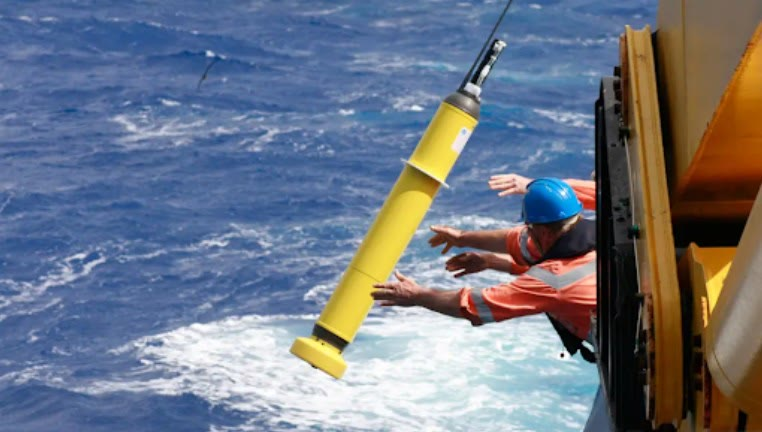
\includegraphics[width=\linewidth]{images/book5/b3-argo-deploy.jpg}

{\scriptsize Pelampung Argo diturunkan dari sisi kapal riset (Program Pemantauan dan
Observasi Samudra Global NOAA, domain publik).}
\end{minipage}
\end{inthefield}
% ledger: argo:fleet, noaa:argo-25, photo:b3-argo-deploy

\section{Pasang surut laut}\label{sec:b3:ocean-dynamics:tides}

Dua kali sehari, dengan selisih sedikit kurang dari satu jam setiap hari, permukaan laut naik dan
turun. Buku fisika menjelaskan gaya pasang surut: tarikan Bulan lebih kuat
di sisi Bumi yang dekat dibanding di pusatnya, dan lebih lemah di sisi
yang jauh, sehingga relatif terhadap pusat, air tertarik keluar sepanjang
garis ke Bulan di kedua sisi.

\begin{definition}[Pasang setimbang; konstituen pasang surut]\label{def:b3:ocean-dynamics:tides}
Yang disebut \emph{pasang setimbang}\index{pasang setimbang} adalah bentuk yang
akan diambil permukaan samudra yang menutupi seluruh Bumi jika mengikuti
potensial pembangkit pasang secara seketika, tanpa inersia. Adapun \emph{konstituen
pasang surut}\index{konstituen pasang surut} adalah salah satu suku harmonik, masing-masing
dengan frekuensi tetap yang ditentukan oleh gerak Bulan dan Matahari serta
amplitudo dan fase yang ditemukan di setiap tempat, yang jumlahnya membentuk pasang surut;
konstituen-konstituen itu diberi nama dengan huruf dan jumlah siklus per hari, misalnya M$_2$,
konstituen semidiurnal lunar utama.
\end{definition}

\begin{theorem}[Pasang setimbang Bulan]\label{thm:b3:ocean-dynamics:equilibrium-tide}
Untuk Bulan, dengan massa $M$ pada jarak $d$ dari pusat Bumi, dengan
massa $M_E$ dan jari-jari $a$, \omterm{def:b3:ocean-dynamics:tides}{pasang setimbang} pada sudut $\theta$ dari
titik di bawah Bulan adalah
\[
\eta = K\,\frac{3\cos^2\theta - 1}{2},\qquad
K = \frac{M}{M_E}\Big(\frac{a}{d}\Big)^3 a .
\]
\end{theorem}

\begin{proof}
Potensial Bulan di suatu titik yang berjarak $a$ dari
pusat Bumi dan sudut $\theta$ adalah $-GM/s$, dengan $s^2 = d^2 - 2ad\cos\theta +
a^2$. Dengan menguraikan dalam $a/d$, $1/s = (1/d)[1 + (a/d)\cos\theta + (a/d)^2
(3\cos^2\theta - 1)/2 + \cdots]$. Suku pertama adalah konstanta; suku kedua
adalah medan seragam, yang mempercepat seluruh Bumi dalam orbitnya
mengelilingi pusat massa bersama, dan tidak berpengaruh terhadap Bumi.
Yang tersisa adalah potensial pembangkit pasang $\Phi_T = -(GMa^2/d^3)(3
\cos^2\theta - 1)/2$. Dalam kesetimbangan, permukaan laut adalah permukaan
potensial total yang konstan, $g\eta + \Phi_T = C$, dengan $g = GM_E/a^2$, sehingga
$\eta = (M/M_E)(a^4/d^3)(3\cos^2\theta - 1)/2 + C/g$. Rata-rata dari
$3\cos^2\theta - 1$ pada seluruh bola adalah nol; karena volume air
tetap, $C = 0$.
\end{proof}

Dengan rasio massa $0.0123$, $d = \qty{384400}{km}$ dan $a =
\qty{6371}{km}$, $K = \qty{0.357}{m}$: permukaan laut berada \qty{0.36}{m}
lebih tinggi di bawah Bulan dan di sisi seberangnya, dan \qty{0.18}{m} lebih rendah pada
lingkaran besar di antaranya, dengan rentang \qty{0.54}{m}. Pada lintang $\varphi$, dengan
Bulan pada deklinasi $\delta$ dan sudut jam $H$, $\cos\theta =
\sin\varphi\sin\delta + \cos\varphi\cos\delta\cos H$. Saat Bumi berputar
di bawah kedua tonjolan, suatu tempat melewati dua air tinggi dalam satu hari lunar,
\qty{24}{h} \qty{50}{min}: pasang surut semidiurnal. Ketika Bulan berada
di utara atau selatan khatulistiwa, kedua tonjolan miring, dan dua air tinggi
dalam sehari tidak sama, seperti tampak pada gambar di bawah. Matahari membangkitkan
pasang dengan bentuk yang sama, \num{0.46} kali lebih besar; keduanya saling menambah saat bulan baru dan
purnama, pada pasang perbani, dan sebagian saling meniadakan pada fase perempat.
% ledger: moon5:orbit, earth:Rmean, stewart:tide-equilibrium (computed in figdata/bachelor-3/tides.py)

\begin{omfigure}
\begin{tikzpicture}
\begin{groupplot}[group style={group size=2 by 1, horizontal sep=1.9cm},
  tick label style={font=\scriptsize}, label style={font=\small},
  legend style={font=\scriptsize, draw=none, fill=none}]
\nextgroupplot[width=0.40\linewidth, height=0.40\linewidth, axis equal image, hide axis,
  clip=false, xmin=-1.3, xmax=2.0, ymin=-1.25, ymax=1.25]
% computed in figdata/bachelor-3/tides.py
\addplot[fill=omThm!12, draw=omThm, thick] table[x=x, y=y] {figdata/out/bachelor-3-tides-bulge.dat};
\addplot[black, fill=black!10, domain=0:360, samples=91] ({cos(x)}, {sin(x)});
\draw[->, >=stealth, thick] (axis cs:1.25,0) -- (axis cs:1.95,0);
\node[above, font=\scriptsize, align=center] at (axis cs:1.6,0.08) {ke\\Bulan};
\node[font=\scriptsize] at (axis cs:0,0) {Bumi};
\nextgroupplot[width=0.54\linewidth, height=0.40\linewidth, xlabel={waktu (\unit{h})},
  ylabel={$\eta$ (\unit{m})}, xmin=0, xmax=49.6, xtick={0,12,24,36,48}, ymin=-0.2, ymax=0.4,
  legend style={at={(axis cs:12.4,0.39)}, anchor=north}, legend cell align=left, legend columns=2]
\addplot[omDef, thick] table[x=t, y=eta0] {figdata/out/bachelor-3-tides-series.dat};
\addlegendentry{$\delta = 0$}
\addplot[omThm, thick] table[x=t, y=eta20] {figdata/out/bachelor-3-tides-series.dat};
\addlegendentry{$\delta = \ang{20}$}
\addplot[black!50, thin, forget plot] coordinates {(0,0) (49.6,0)};
\end{groupplot}
\end{tikzpicture}

\par\smallskip{\small Kiri, \omterm{def:b3:ocean-dynamics:tides}{pasang setimbang} Bulan, pada bidang
yang memuat Bulan, tonjolan dibesar-besarkan sekitar dua juta kali.
Kanan, \omterm{def:b3:ocean-dynamics:tides}{pasang setimbang} pada \ang{45} LU selama dua hari lunar, dengan
Bulan di khatulistiwa (biru) dan pada deklinasi \ang{20} LU (merah): kasus kedua
memiliki satu air tinggi jauh lebih tinggi daripada yang lain, ketaksamaan
diurnal.}\label{fig:b3:ocean-dynamics:equilibrium-tide}
\end{omfigure}
% ledger: moon5:orbit, stewart:tide-constituents

Analisis harmonik \omterm{def:b3:ocean-dynamics:tides}{pasang setimbang} menghasilkan konstituennya. Lima
konstituen terbesar, dengan amplitudo setimbangnya, tercantum pada tabel di bawah.
Setidaknya 39 konstituen diperlukan untuk memprediksi pasang surut pelabuhan hingga seperseribu dari
suku terbesarnya, dan pengukur pasang harus beroperasi lebih dari 18.6 tahun, periode
modulasi pasang lunar, untuk memisahkan seluruhnya.

\begin{center}
\small
\begin{tabular}{llrr}
\hline
konstituen & asal & periode (\unit{h}) & amplitudo setimbang (\unit{m}) \\
\hline
M$_2$ & lunar utama, semidiurnal & \num{12.4206} & \num{0.2423} \\
S$_2$ & solar utama, semidiurnal & \num{12.0000} & \num{0.1128} \\
N$_2$ & lunar eliptik, semidiurnal & \num{12.6584} & \num{0.0464} \\
K$_1$ & lunisolar, diurnal & \num{23.9344} & \num{0.1416} \\
O$_1$ & lunar utama, diurnal & \num{25.8194} & \num{0.1005} \\
\hline
\end{tabular}
\end{center}
% ledger: stewart:tide-constituents, stewart:tide-prediction

Pasang surut sebenarnya bukan \omterm{def:b3:ocean-dynamics:tides}{pasang setimbang}. Agar tonjolan tetap berada di bawah Bulan
di khatulistiwa, pasang harus merambat mengelilingi Bumi dalam satu hari lunar,
dengan laju sekitar \qty{460}{m/s}, kecepatan yang hanya dicapai gelombang gravitasi panjang
di samudra dengan kedalaman \qty{22}{km}; dan benua menghentikannya. Pasang surut
justru adalah gelombang panjang paksa, yang berayun di tiap cekungan dekat resonansi, dan
rotasi Bumi membuatnya berputar mengelilingi cekungan.
% ledger: stewart:tide-prediction

\begin{definition}[Gelombang Kelvin]\label{def:b3:ocean-dynamics:kelvin-wave}
Yang disebut \emph{gelombang Kelvin}\index{gelombang Kelvin} di samudra adalah gelombang gravitasi panjang
yang merambat sepanjang pesisir atau sepanjang khatulistiwa, tanpa kecepatan melintang
terhadapnya, tingginya menurun secara eksponensial menjauhi pesisir sepanjang
jari-jari Rossby. Sepanjang pesisir ia merambat dengan pesisir di sisi kanannya pada
belahan bumi utara, dan di sisi kirinya pada belahan bumi selatan.
\end{definition}

\begin{theorem}[Gelombang Kelvin pesisir]\label{thm:b3:ocean-dynamics:kelvin}
Di samudra dengan kedalaman seragam $H$ pada bidang-$f$, dengan $f > 0$, yang dibatasi oleh
pesisir lurus sepanjang $y = 0$ dan berada di $y > 0$, persamaan air dangkal linear
memiliki solusi dengan $v = 0$
\[
\eta = \mathrm e^{-y/L_R}F(x - ct),\qquad u = \frac{g}{c}\,\eta,\qquad
c = \sqrt{gH},\quad L_R = \frac{c}{f},
\]
untuk sembarang profil $F$, dan tidak ada solusi dengan $v = 0$ yang merambat ke arah
$-x$.
\end{theorem}

\begin{proof}
Dengan $v = 0$ persamaannya adalah $\partial u/\partial t = -g\,\partial\eta/
\partial x$, $fu = -g\,\partial\eta/\partial y$ dan $\partial\eta/\partial t
+ H\,\partial u/\partial x = 0$. Persamaan pertama dan ketiga memberikan $\partial^2
\eta/\partial t^2 = gH\,\partial^2\eta/\partial x^2$: dalam $x$ setiap garis
$y = $ konstan memuat gelombang $F(x \mp ct)$ dengan $c = \sqrt{gH}$, dan kemudian persamaan
pertama memberikan $u = \pm(g/c)\eta$. Persamaan kedua menjadi $\partial\eta/
\partial y = \mp(f/c)\eta$, sehingga $\eta \propto \mathrm e^{\mp y/L_R}$. Untuk
tanda atas gelombang meluruh menjauhi pesisir; untuk tanda bawah ia
akan tumbuh tanpa batas ke arah samudra, yang tidak mungkin. Gelombang merambat
ke arah $+x$ dengan samudra di sisi kirinya dan pesisir di sisi kanannya.
\end{proof}

Di samudra dalam, dengan kedalaman \qty{4000}{m}, $c = \qty{198}{m/s}$ dan
jari-jari Rossby sekitar \qty{2000}{km} di lintang tengah: pasang surut menyapu
seluruh cekungan. Di laut paparan dengan kedalaman \qty{50}{m}, $c =
\qty{22}{m/s}$, jari-jari Rossby kurang dari \qty{200}{km}, dan panjang gelombang M$_2$
sekitar \qty{1000}{km}. Di teluk, pasang surut yang masuk sepanjang satu
pesisir sebagai \omterm{def:b3:ocean-dynamics:kelvin-wave}{gelombang Kelvin} kembali sepanjang pesisir seberangnya, lagi-lagi dengan
pesisir di sisi kanannya; kedua gelombang saling meniadakan di titik-titik di antaranya.

\begin{definition}[Titik amfidromik; garis kotidal; garis ko-rentang]\label{def:b3:ocean-dynamics:amphidrome}
Yang disebut \emph{titik amfidromik}\index{titik amfidromik} adalah titik tempat
amplitudo suatu \omterm{def:b3:ocean-dynamics:tides}{konstituen pasang surut} bernilai nol dan air tinggi di sekitarnya
berputar. Sebuah \emph{garis kotidal}\index{garis kotidal} menghubungkan tempat-tempat yang
air tinggi suatu konstituen tiba pada waktu yang sama; sedangkan \emph{garis
ko-rentang}\index{garis ko-rentang} menghubungkan tempat-tempat dengan rentang pasang surut yang sama.
Garis kotidal memancar dari titik amfidromik; garis ko-rentang mengelilinginya.
\end{definition}

\begin{omfigure}
\centering
\begin{tikzpicture}
\begin{axis}[width=0.96\linewidth, height=0.35\linewidth, axis equal image,
  xmin=0, xmax=1600, ymin=0, ymax=400, xtick={0,400,800,1200,1600}, ytick={0,200,400},
  xlabel={jarak sepanjang alur (\unit{km})}, ylabel={melintang (\unit{km})},
  tick label style={font=\scriptsize}, label style={font=\small}]
% computed in figdata/bachelor-3/tides.py
\addplot[omDef!70, densely dashed, unbounded coords=jump] table[x=x, y=y] {figdata/out/bachelor-3-tides-cor.dat};
\pgfplotsinvokeforeach{30,60,90,120,150,180,210,240,270,300,330}{
  \addplot[omThm, thin, unbounded coords=jump] table[x=x, y=y] {figdata/out/bachelor-3-tides-cot-#1.dat};
}
\addplot[omThm, very thick, unbounded coords=jump] table[x=x, y=y] {figdata/out/bachelor-3-tides-cot-0.dat};
\addplot[only marks, mark=*, mark size=2pt] table[x=x, y=y] {figdata/out/bachelor-3-tides-amph.dat};
\addplot[->, >=stealth, very thick, domain=20:310, samples=60] ({742.7+70*cos(x)}, {200+70*sin(x)});
\end{axis}
\end{tikzpicture}

\par\smallskip{\small Dua \omterm{def:b3:ocean-dynamics:kelvin-wave}{gelombang Kelvin} pasang surut M$_2$ dalam sebuah alur rekaan
selebar \qty{400}{km} dan sedalam \qty{50}{m} pada \ang{55} LU, satu merambat
ke timur sepanjang pesisir selatan, yang lain ke barat sepanjang pesisir utara.
Merah, garis-garis kotidal setiap \ang{30} fase (sekitar satu jam), yang
tebal untuk air tinggi pada titik awal waktu; biru putus-putus, \omterm{def:b3:ocean-dynamics:amphidrome}{garis ko-rentang}
setiap seperlima amplitudo satu gelombang di pesisirnya. \omterm{def:b3:ocean-dynamics:amphidrome}{Titik
amfidromik} (titik-titik) terletak pada garis tengah, berjarak setengah panjang gelombang,
yakni \qty{495}{km}, dan air tinggi berputar mengelilinginya berlawanan arah jarum jam
(panah).}\label{fig:b3:ocean-dynamics:amphidromes}
\end{omfigure}

Peta pasang surut samudra yang dibuat dari altimetri satelit, akurat hingga sekitar
\qty{2}{cm} di laut dalam, menunjukkan struktur ini di mana-mana: puncak M$_2$
berputar berlawanan arah jarum jam mengelilingi \omterm{def:b3:ocean-dynamics:amphidrome}{titik amfidromik} cekungan belahan bumi utara
dan searah jarum jam di belahan bumi selatan, dan rentang terbesar berada di
pesisir. Pasang surut mendisipasikan \qty{3.75}{TW}, dan \qty{3.5}{TW} di antaranya di
samudra, sekitar dua pertiga energi M$_2$ terdisipasi di paparan dan laut dangkal, dan
sepertiga melalui gelombang internal di samudra dalam. Energi itu
memperpanjang hari sekitar \qty{2.07}{ms} per abad dan mendorong Bulan menjauh
sejauh \qty{3.86}{cm} per tahun; dan bagian yang hilang di samudra dalam mengaduknya,
menyediakan sebagian pengadukan yang, dalam gambaran Stommel--Arons, menggerakkan
sirkulasi abisal.
% ledger: stewart:tide-prediction


\section{Latihan}

\begin{exercise}[$\star$]\label{exo:b3:ocean-dynamics:1}
Tegangan angin dari arah barat sebesar \qty{0.12}{Pa} bertiup di atas laut pada \ang{40} LU
($\rho = \qty{1025}{kg/m^3}$, $\Omega = \qty{7.292115e-5}{rad/s}$).
Hitung transpor volume Ekman per meter lebar dan arahnya,
serta transpor melintasi penampang sepanjang \qty{1000}{km}, dalam sverdrup.
\end{exercise}

\begin{exercise}[$\star$]\label{exo:b3:ocean-dynamics:2}
Dengan $A_z = \qty{0.05}{m^2/s}$, hitung \omterm{def:b3:ocean-dynamics:ekman-pumping}{kedalaman Ekman} pada \ang{45} LU. Berapa
bagian arus permukaan yang tersisa pada kedalaman itu?
\end{exercise}

\begin{exercise}[$\star$]\label{exo:b3:ocean-dynamics:3}
Pada \ang{30} LU, kurl tegangan angin bernilai \qty{-1e-7}{Pa/m} di seluruh
cekungan selebar \qty{5000}{km} ($a = \qty{6371}{km}$). Hitung $\beta$, transpor
Sverdrup per satuan lebar, dan transpor total beserta
arahnya.
\end{exercise}

\begin{exercise}[$\star$]\label{exo:b3:ocean-dynamics:4}
Dari periode M$_2$ dan S$_2$, hitung periode siklus pasang purnama
dan pasang perbani, yakni waktu antara dua penjajaran dari kedua
konstituen tersebut.
\end{exercise}

\begin{exercise}[$\star\star$]\label{exo:b3:ocean-dynamics:5}
Tegangan angin baratan bertambah secara linear dari 0 pada \ang{35} LU hingga \qty{0.1}{Pa} pada
\ang{45} LU, \qty{1110}{km} lebih ke utara. Hitung \omterm{def:b3:ocean-dynamics:ekman-pumping}{pemompaan Ekman} pada
\ang{40} LU dengan mempertahankan kedua suku pada \cref{prop:b3:ocean-dynamics:pumping},
dalam meter per tahun. Apakah air didorong naik atau turun?
\end{exercise}

\begin{exercise}[$\star\star$]\label{exo:b3:ocean-dynamics:6}
Dalam gyre Stommel dengan $r = \qty{2e-6}{s^{-1}}$ dan $\beta =
\qty{2e-11}{m^{-1}.s^{-1}}$, hitung lebar $\delta_S$. Jika arus batas
membawa \qty{30}{\sverdrup} di \qty{800}{m} teratas, dalam
lebar $\delta_S$, berapa kelajuan rata-ratanya?
\end{exercise}

\begin{exercise}[$\star\star$]\label{exo:b3:ocean-dynamics:7}
Hitung lebar Munk $\delta_M$ dan lebar pancaran ke utara,
$(2\pi/\sqrt3)\,\delta_M$, pada \ang{30} LU untuk $A_H = \qty{e4}{m^2/s}$. Bagaimana
lebar itu berubah jika $A_H$ delapan kali lebih kecil?
\end{exercise}

\begin{exercise}[$\star\star$]\label{exo:b3:ocean-dynamics:8}
Dua stasiun berjarak \qty{80}{km} terletak pada garis dari barat ($A$) ke timur
($B$) pada \ang{36} LU. Relatif terhadap permukaan \qty{1000}{dbar}, anomali
\omterm{def:b3:gravity-geodesy:geopotential}{geopotensial} permukaan laut bernilai \qty{14.5}{J/kg} di $A$ dan
\qty{21.3}{J/kg} di $B$. Hitung arus permukaan relatif terhadap
\qty{1000}{dbar} beserta arahnya. Stasiun mana yang memiliki kolom
air yang lebih hangat?
\end{exercise}

\begin{exercise}[$\star\star$]\label{exo:b3:ocean-dynamics:9}
Dengan \omterm{def:b3:ocean-dynamics:tides}{pasang setimbang} Bulan, $K = \qty{0.357}{m}$, dan rasio
\num{0.46} antara pasang Matahari dan pasang Bulan, hitung rentang
\omterm{def:b3:ocean-dynamics:tides}{pasang setimbang} (air tinggi di bawah benda langit dikurangi air rendah pada \ang{90}) saat pasang purnama dan
pasang perbani, serta rasionya.
\end{exercise}

\begin{exercise}[$\star\star\star$]\label{exo:b3:ocean-dynamics:10}
Pada bidang-$\beta$ khatulistiwa, $f = \beta_0y$ dengan $\beta_0 =
2\Omega/a$. Tunjukkan bahwa \omterm{def:b3:ocean-dynamics:kelvin-wave}{gelombang Kelvin} $\eta = G(y)F(x - ct)$, $v = 0$,
menjadi $G = \exp(-\beta_0y^2/2c)$, terperangkap di kedua sisi khatulistiwa,
dan merambat ke timur. Hitung skala perangkapannya $\sqrt{c/\beta_0}$ untuk
gelombang dengan kelajuan \qty{2.5}{m/s}.
\end{exercise}

\begin{exercise}[$\star\star\star$]\label{exo:b3:ocean-dynamics:11}
(a)~Turunkan $V = a\tan\varphi\,W_0$ untuk interior abisal dari $\beta v =
f\,\partial w/\partial z$. (b)~Dengan $W_0 = \qty{e-7}{m/s}$, hitung $V$ pada
\ang{30} LU serta transpor total ke kutub melintasi cekungan
selebar \qty{5000}{km}. (c)~Dari mana air itu harus berasal?
\end{exercise}

\begin{exercise}[$\star\star\star$]\label{exo:b3:ocean-dynamics:12}
Arus geostrofik $W_g = u_g + \mathrm iv_g$ mengalir di atas dasar laut
datar pada $z = 0$, dengan viskositas \omterm{def:b3:atmospheric-dynamics:eddy}{eddy} $A_z$ dan tanpa slip di dasar.
(a)~Tunjukkan bahwa $W = W_g(1 - \mathrm e^{-(1+\mathrm i)z/\delta})$, $\delta =
\sqrt{2A_z/f}$. (b)~Tunjukkan bahwa defisit transpor lapisan Ekman dasar ini
memompa kecepatan vertikal $w = \tfrac12\delta\zeta_g$ ke dalam
interior, $\zeta_g$ vortisitas arus geostrofik. (c)~Untuk
$A_z = \qty{0.01}{m^2/s}$, $f = \qty{e-4}{s^{-1}}$, dan samudra
berkedalaman \qty{4000}{m}, hitung $\delta$, laju peluruhan putaran $r =
f\delta/2H$, serta kebalikannya dalam hari.
\end{exercise}
% ledger: earth:Rmean, geod5:grs80-defining, stewart:tide-constituents, stewart:tide-equilibrium

\section{Soal: Gyre di Laut Ammar}

\begin{problem}[{Soal akhir pekan --- pemompaan Ekman, transpor Sverdrup,
arus batas barat dan pasang surut samudra rekaan}]
\label{pb:b3:ocean-dynamics:1}
Laut Ammar adalah cekungan samudra rekaan, berbentuk persegi panjang dari \ang{20} hingga
\ang{50} LU dan selebar \qty{6000}{km}, dengan kedalaman \qty{4000}{m}. Tegangan angin bersifat
zonal, $\tau_x = -\tau_0\cos(\pi(\varphi - \ang{20})/\ang{30})$ dengan $\tau_0
= \qty{0.1}{Pa}$. Gunakan $\rho = \qty{1025}{kg/m^3}$, $\Omega =
\qty{7.292115e-5}{rad/s}$, $a = \qty{6371}{km}$, $g = \qty{9.81}{m/s^2}$,
dan, jika bidang-$\beta$ diminta, nilainya pada \ang{35} LU.

\medskip\noindent\textbf{Bagian I --- Lapisan Ekman.}
\begin{enumerate}
\item Hitung tegangan angin pada \ang{20}, \ang{35}, dan \ang{50} LU.
\item Hitung $f$ pada lintang yang sama.
\item Hitung transpor volume Ekman per satuan lebar pada \ang{20} dan
  \ang{50} LU, beserta arahnya. Apakah transpor itu konvergen atau divergen di
  cekungan?
\item Dengan $A_z = \qty{0.05}{m^2/s}$, hitung \omterm{def:b3:ocean-dynamics:ekman-pumping}{kedalaman Ekman} pada \ang{35} LU.
\item Hitung \omterm{def:b3:ocean-dynamics:ekman-pumping}{pemompaan Ekman} pada \ang{35} LU, dalam meter per detik dan per
  tahun.
\item Berapa tahun yang dibutuhkan pemompaan ini untuk mendorong air permukaan
  ke bawah sejauh \qty{500}{m}?
\end{enumerate}

\medskip\noindent\textbf{Bagian II --- Interior Sverdrup.}
\begin{enumerate}[resume]
\item Hitung panjang $L$ cekungan dari selatan ke utara dan $\beta$ pada
  \ang{35} LU.
\item Hitung kurl tegangan angin pada \ang{35} LU.
\item Hitung transpor Sverdrup per satuan lebar pada \ang{35} LU, beserta
  arahnya.
\item Hitung transpor interior total melintasi cekungan pada \ang{35} LU,
  dalam sverdrup.
\item Jika aliran ini tersebar di \qty{1000}{m} teratas, berapa kelajuan rata-ratanya,
  dan berapa tahun yang dibutuhkan sebuah parsel air untuk bergerak sejauh \qty{1000}{km}
  ke selatan?
\item Tunjukkan bahwa $fw_E/\beta$ pada \ang{35} LU memberikan transpor yang sama, dan
  jelaskan mengapa dengan \omterm{def:b3:atmospheric-dynamics:pv}{vortisitas potensial} sebuah kolom.
\end{enumerate}

\medskip\noindent\textbf{Bagian III --- Arus batas barat.}
\begin{enumerate}[resume]
\item Jelaskan mengapa aliran balik tidak dapat mengalir di sepanjang sisi timur
  cekungan.
\item Dengan gesekan dasar $r = \qty{e-6}{s^{-1}}$, hitung
  lebar Stommel $\delta_S$.
\item Hitung transpor ke utara per satuan lebar pada dinding barat,
  $A(X/\delta_S - 1)$, serta kelajuan rata-rata jika mengisi lapisan
  \qty{1000}{m} teratas.
\item Seberapa jauh dari dinding aliran ke utara berakhir?
\item Hitung transpor ke utara lapisan batas Stommel, dan
  jelaskan mengapa transpor itu lebih kecil daripada transpor interior sekitar
  \qty{1.5}{\sverdrup}.
\item Dengan $A_H = \qty{5e3}{m^2/s}$, hitung $\delta_M$ dan lebar
  pancaran Munk ke utara.
\item Pancaran Munk membawa $1 + \mathrm e^{-\pi/\sqrt3}$ kali
  transpor interior. Hitung besarnya, dan katakan ke mana kelebihannya pergi.
\end{enumerate}

\medskip\noindent\textbf{Bagian IV --- Pasang surut Laut Ammar.}
\begin{enumerate}[resume]
\item Hitung kelajuan \omterm{def:b3:ocean-dynamics:kelvin-wave}{gelombang Kelvin} di cekungan dan jari-jari Rossby
  pada \ang{35} LU.
\item Hitung panjang \omterm{def:b3:ocean-dynamics:kelvin-wave}{gelombang Kelvin} M$_2$.
\item Berapa lama \omterm{def:b3:ocean-dynamics:kelvin-wave}{gelombang Kelvin} merambat sekali mengelilingi pesisir
  cekungan, dan berapa periode M$_2$ yang setara dengan waktu itu?
\item Dengan kelajuan berapa \omterm{def:b3:ocean-dynamics:tides}{pasang setimbang} harus bergerak mengelilingi
  lingkaran \ang{35} LU agar tetap berada di bawah Bulan, dan pada kedalaman samudra berapa
  gelombang panjang akan merambat secepat itu?
\item Di mana kamu perkirakan \omterm{def:b3:ocean-dynamics:amphidrome}{titik amfidromik} cekungan, dan ke arah mana
  air tinggi berputar mengelilinginya?
\item Hitung amplitudo setimbang semidiurnal pada \ang{35} LU, $\tfrac34
  K\cos^2\varphi$, dengan $K = \qty{0.357}{m}$, untuk Bulan di khatulistiwa.
\item Berikan transpor arus batas barat yang menutup
  gyre Laut Ammar.
\end{enumerate}
\end{problem}
% ledger: earth:Rmean, geod5:grs80-defining, stewart:tide-constituents
